\documentclass{article}
\usepackage[english]{babel}
\usepackage[utf8]{inputenc}
\usepackage[T1]{fontenc}
\usepackage{graphicx}
\usepackage{caption}
\usepackage{subcaption}
\usepackage{float}
\usepackage{wrapfig}
\usepackage{setspace}
\usepackage{cite}
\usepackage{url}
\usepackage{color}
\definecolor{linkcol}{rgb}{0,0,0.4}
\definecolor{citecol}{rgb}{0.5,0,0}
\usepackage[pagebackref,hyperindex=true]{hyperref}
\hypersetup{colorlinks=true,linkcolor=linkcol,citecolor=citecol,urlcolor=linkcol}

\usepackage{listings}
\lstset{
    language=C++,
    basicstyle=\ttfamily\small,
    aboveskip={1.0\baselineskip},
    belowskip={1.0\baselineskip},
    columns=fixed,
    extendedchars=true,
    breaklines=true,
    tabsize=4,
    prebreak=\raisebox{0ex}[0ex][0ex]{\ensuremath{\hookleftarrow}},
    frame=lines,
    showtabs=false,
    showspaces=false,
    showstringspaces=false,
    keywordstyle=\bfseries,
    commentstyle=\color[rgb]{0.133,0.545,0.133},
    stringstyle=\color[rgb]{01,0,0},
    numbers=none,
    numberstyle=\small,
    stepnumber=1,
    numbersep=10pt,
    captionpos=b,
    escapeinside={\%*}{*)}
}

\begin{document}

\begin{titlepage}
\begin{center}
  \hfill
  \vspace{3.0cm}

  {\huge \textsc{IO Operations for wavepackets with HDF5 Interface in C++\\[10pt]
  }}
  ~\\[20pt]

  {\huge{Bachelor Thesis}}\\[2.5cm]

  {\emph{written by}}\\
  Florian Frei
  \\[0.6cm]
  {\emph{supervised by}}\\
  Dr. Vasile Gr\u{a}dinaru\\
  {\emph{and}}\\
  Prof. Dr. Ralf Hiptmair
  \\[2.5cm]

  Seminar for Applied Mathematics\\
  ETH Zurich
  \\[0.5cm]
  \emph{{Spring semester 2016}}
\end{center}
\end{titlepage}



\tableofcontents
\clearpage

\section{Introduction}
This thesis is about the continuation of the C++ implementation \cite{libwaveblocks} and allows a comparison to the Python implementation \cite{waveblocksnd}. The already existing framework is sufficient to generate simulations of different kind of Hagedorn wavepackets. The data produced is written in HDF5 binary format whereas the data from the C++ implementation is not easily comparable to the generated data from python. The writing process in the C++ implementation is currently done by using an extern project \cite{eigen3-hdf5}. The new implementation for writing binary HDF format in C++ will be explained in this thesis and also the new implementation allows easy comparison between Python and C++. It also incorporates a testing file which takes two HDF binary data files as arguments and compares the coinciding data. The testing file uses the well-known GoogleTest interface\cite{googletest}.

\section{HDF5 C++ Interface}
HDF stands for hierarchical data format which allows internal structure similar to a file system.
\subsection{Overview}
From the documentation we can conclude that the C++ interface is just a nice wrapper of the C interface. The corresponding classes and wrappers are shown in the following table:\\
\\
\begin{tabular}{|l|l|}
\hline
HDF5 C APIs&C++ Classes\\
\hline
Attribute Interface (H5A)&Attribute\\
Datasets Interface (H5D)&DataSet\\
Error Interface (H5E)&Exception\\
File Interface (H5F)&H5File\\
Group Interface(H5G)&Group\\
Identifier Interface (H5I)&IdComponent\\
Property List Interface (H5P)&PropList and subclasses\\
Dataspace Interface (H5S)&DataSpace\\
Datatype Interface (H5T)&DataType and subclasses\\
\hline
\end{tabular}\\
\\
The hierarchy of these classes is depicted in the following diagramm:\\
\begin{figure}[H]
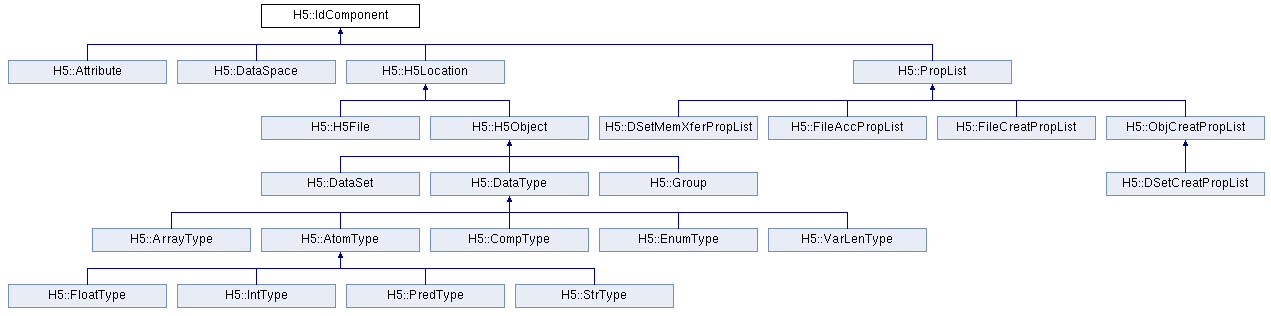
\includegraphics[scale=0.39]{inheritance_diagramm.png}
\caption{Inheritance diagram of IdComponent}
\end{figure}

Throughout this thesis we will ignore the "H5" namespace and will always directly refer to the name of the object.\\
For our purposes we need to save a Hagedorn wave packet in every time step which consists of matrices and vectors. For these we need a DataSpace which allows us to write matrices and vectors in a time-dimension. In our case the time-dimension is arbitrarily chosen depending on the kind of the simulation. As such we need a DSetCreatePropList which is used to describe properties such as chunk-dimension for matrices used in our case for time-dimension. Attribute are used to save additional information such as the used time-step $\delta t$ in the simulation. For constructing a HDF5 binary file we need to use the File class which simply uses a string argument as the filename. For neatness we want to have a intern structure for our data. For this we use the Group class which is very similar to the file system and its folders for structuring. To write Eigen-matrices we need the DataType class which defines how to write these data types. Last but not least we need a DataSet for every object we want to write to our binary file.

\subsection{Intern used data-types}
Often we make function calls with arguments to the HDF5 library. These arguments have to be of an intern data type which the library expects. For our needs we mostly need hsize\_t and H5std\_string and every class mentioned in the previous section.
\subsubsection{hsize$\_$t}
Variables of this type represent native multiple-precision integer. 
\subsubsection{H5std$\_$string}
H5std\_string is just an alias for the std::string type.
\subsection{DataType}
The DataType class describes how to write different kind of types and handles writing options. Every DataType is given a name which is stored in a string used as its representation. As we can see from the previous figure DataType is derived from H5Object and is further decomposable in ArrayType, AtomType, CompType, EnumType and VarLenType. For example when we want to write a native double and we don't care how it is represented on our system we would use a PredType from AtomType because it will use the definition from the operating system. When we would like to choose or define ourself how to write a double we would use the FloatType from AtomType. For cases where our data type is a struct of atomic types we would use the a CompType. For interested parties and further explanations we refer to the HDF5 official documentation\cite{hdf5doc}.
\subsection{DataSpace}
To write in a DataSet the HDF5-library needs minimal four arguments. First is a pointer to the buffer of the source. Second is the type which is written. Third and fourth is the source and destination space respectively. There can be additional arguments such as which compression should be used for writing. The third and fourth arguments needs to of type DataSpace. A simple way to construct such a DataSpace is to call the constructor with two arguments. The first one is the rank of the space, which indicates the number of dimension the space will have. Following as the second argument is an array of type hsize\_t with size of the previous used rank with the number of elements in each dimension. For example for a time grid DataSpace the following code is sufficient:\\

\begin{lstlisting}
const int RANK = 1;
hsize_t size[RANK];
size[0]=number_of_timesteps;
\end{lstlisting}

The problem herein lies in the number of time steps which is unknown when we construct our DataSpace. This leads to another approach which is to extend continuously which will be explained later on.
\subsection{DataSet}
A DataSet is used as the location and representation for an object of interest which will be written. To construct a DataSet we need four arguments. First argument is a string which represents the name and also the inner location in the file. The second argument describes the used DataType to write data to this set. The third argument is a DataSpace which describes the dimension of the DataSet. The forth and last argument is a DSetCreatPropList which describes inner properties of the DataSet for example the default fill value or the extensibility of the set.
\subsection{Attribute}
An Attribute is used to write additional information to an existing Group oder DataSet. To create an Attribute we need three arguments. First is a string for the name of the attribute. Second is the used type of the Attribute. Third and last is the DataSpace of the attribute. In our case we want to add an Attribute to the root Group "/" which has the name "dt" and is used to indicate the time step in this simulation.
\subsection{DSetCreatePropList}
We use a DSetCreatPropList to change the properties of writing to the DataSet. At start a DataSet is always of simple but this doesn't allow us easy extension of the DataSet. For our purpose we use the setChunk function to change this property. To construct such an object no additional arguments are needed and we can use just the default one.
\subsection{Group}
We use Groups to further structure our data in the file. Suppose we have a Hagedorn wavepacket and the corresponding energy with a time series then we would like to structure these in the file in a sub folder manner such as "/wavepacket/Pi/*" for the packet, "/wavepacket/timegrid" for its time series and "/observables/energies/*" for the energy and its time series. It is straightforward that for every sub folder one needs a new Group. 
\subsection{File}

\section{Eigen Interface}

\section{HDF5 Writer template}

\section{Datatest with GoogleTest Framework}
\subsection{Initialization}
\subsection{Testfissure}
\subsection{Testclass including HDF5 Interface}


%\nocite{*}


\bibliographystyle{plain}
\bibliography{references,wp,own}

\end{document}
